\documentclass[journal,12pt,twocolumn]{IEEEtran}

\usepackage{setspace}
\usepackage{gensymb}
\singlespacing
\usepackage[cmex10]{amsmath}

\usepackage{amsthm}

\usepackage{mathrsfs}
\usepackage{txfonts}
\usepackage{stfloats}
\usepackage{bm}
\usepackage{cite}
\usepackage{cases}
\usepackage{subfig}

\usepackage{longtable}
\usepackage{multirow}
\usepackage{enumitem}
\usepackage{mathtools}
\usepackage{steinmetz}
\usepackage{tikz}
\usepackage{circuitikz}
\usepackage{verbatim}
\usepackage{tfrupee}
\usepackage[breaklinks=true]{hyperref}
\usepackage{graphicx}
\usepackage{tkz-euclide}

\usetikzlibrary{calc,math}
\usepackage{listings}
    \usepackage{color}                                            %%
    \usepackage{array}                                            %%
    \usepackage{longtable}                                        %%
    \usepackage{calc}                                             %%
    \usepackage{multirow}                                         %%
    \usepackage{hhline}                                           %%
    \usepackage{ifthen}                                           %%
    \usepackage{lscape}     
\usepackage{multicol}
\usepackage{chngcntr}

\DeclareMathOperator*{\Res}{Res}

\renewcommand\thesection{\arabic{section}}
\renewcommand\thesubsection{\thesection.\arabic{subsection}}
\renewcommand\thesubsubsection{\thesubsection.\arabic{subsubsection}}

\renewcommand\thesectiondis{\arabic{section}}
\renewcommand\thesubsectiondis{\thesectiondis.\arabic{subsection}}
\renewcommand\thesubsubsectiondis{\thesubsectiondis.\arabic{sub subsection}}


\hyphenation{optical networks semiconduc-tor}
\def\inputGnumericTable{}                                 %%

\lstset{
%language=C,
frame=single, 
breaklines=true,
columns=fullflexible
}
\date{March 2021}

\begin{document}

\newcommand{\BEQA}{\begin{eqnarray}}
\newcommand{\EEQA}{\end{eqnarray}}
\newcommand{\define}{\stackrel{\triangle}{=}}
\bibliographystyle{IEEEtran}
\raggedbottom
\setlength{\parindent}{0pt}
\providecommand{\mbf}{\mathbf}
\providecommand{\pr}[1]{\ensuremath{\Pr\left(#1\right)}}
\providecommand{\qfunc}[1]{\ensuremath{Q\left(#1\right)}}
\providecommand{\fn}[1]{\ensuremath{f\left(#1\right)}}
\providecommand{\e}[1]{\ensuremath{E\left(#1\right)}}
\providecommand{\sbrak}[1]{\ensuremath{{}\left[#1\right]}}
\providecommand{\lsbrak}[1]{\ensuremath{{}\left[#1\right.}}
\providecommand{\rsbrak}[1]{\ensuremath{{}\left.#1\right]}}
\providecommand{\brak}[1]{\ensuremath{\left(#1\right)}}
\providecommand{\lbrak}[1]{\ensuremath{\left(#1\right.}}
\providecommand{\rbrak}[1]{\ensuremath{\left.#1\right)}}
\providecommand{\cbrak}[1]{\ensuremath{\left\{#1\right\}}}
\providecommand{\lcbrak}[1]{\ensuremath{\left\{#1\right.}}
\providecommand{\rcbrak}[1]{\ensuremath{\left.#1\right\}}}
\theoremstyle{remark}
\newtheorem{rem}{Remark}
\newcommand{\sgn}{\mathop{\mathrm{sgn}}}
\providecommand{\abs}[1]{\vert#1\vert}
\providecommand{\res}[1]{\Res\displaylimits_{#1}} 
\providecommand{\norm}[1]{\lVert#1\rVert}
%\providecommand{\norm}[1]{\lVert#1\rVert}
\providecommand{\mtx}[1]{\mathbf{#1}}
\providecommand{\mean}[1]{E[ #1 ]}
\providecommand{\fourier}{\overset{\mathcal{F}}{ \rightleftharpoons}}
%\providecommand{\hilbert}{\overset{\mathcal{H}}{ \rightleftharpoons}}
\providecommand{\system}{\overset{\mathcal{H}}{ \longleftrightarrow}}
	%\newcommand{\solution}[2]{\textbf{Solution:}{#1}}
\newcommand{\solution}{\noindent \textbf{Solution: }}
\newcommand{\cosec}{\,\text{cosec}\,}
\providecommand{\dec}[2]{\ensuremath{\overset{#1}{\underset{#2}{\gtrless}}}}
\newcommand{\myvec}[1]{\ensuremath{\begin{pmatrix}#1\end{pmatrix}}}
\newcommand{\mydet}[1]{\ensuremath{\begin{vmatrix}#1\end{vmatrix}}}
\numberwithin{equation}{subsection}
\makeatletter
\vspace{3cm}
\title{Assignment 3}
\author{Adhvik Mani Sai Murarisetty - AI20BTECH11015}
\maketitle
\newpage
\bigskip
\renewcommand{\thetable}{\theenumi}
Download all python codes from 
\begin{lstlisting}
https://github.com/adhvik24/AI1103-PROBABILITY-AND-RANDOM-VARIABLES/tree/main/ASSIGNMENT%203/codes
\end{lstlisting}
%
and latex-tikz codes from 
%
\begin{lstlisting}
https://github.com/adhvik24/AI1103-PROBABILITY-AND-RANDOM-VARIABLES/tree/main/ASSIGNMENT%203/AI1103_Assignment3.tex
\end{lstlisting}
\section{Gate XE-A-2017-QN 2}
Three fair dies are rolled simultaneously. The probability of getting a sum of 5 is
\begin{enumerate}[label=(\Alph*)]
    \item $\frac{1}{108}$
    \item $\frac{1}{72}$
    \item $\frac{1}{54}$
    \item $\frac{1}{36}$
\end{enumerate}

\section{Solution}
Let
$X_i\in\,$\cbrak{1,2,3,4,5,6}, i = 1,2,3, be the random variables representing the outcome for each die. As the dies are fair, the probability mass function (pmf) is expressed as
\begin{align}
    P_{X_i}(n) = \pr{X_i = n} = 
\begin{cases}
\frac{1}{6} & 1 \le n \le 6
\\
0 & otherwise
\end{cases}\label{1}
\end{align}
Let X be a random variable denotes the desired outcome,
\begin{align}
    X=X_1+X_2+X_3\label{2}\\
    \implies X\in\cbrak{3,4,...,18}
\end{align}
We also know that when two dies are rolled the probability mass function of a random variable Y is (Where Y denotes the sum of values appeared on each die$\implies Y=X_1+X_2$)
\begin{align}
P_Y(n)= 
\begin{cases}
0 & n < 1
\\
\frac{n-1}{36} &  2 \le n \le  7
\\
\frac{13-n}{36} & 7 < n \le 12
\\
0 & n > 12
\end{cases}\label{3}\\
P_Y(n)=\pr{X_1+X_2=n} 
\end{align}
\begin{figure}[htp]
    \centering
    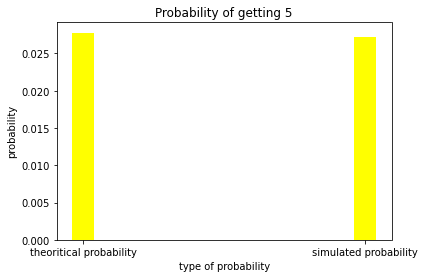
\includegraphics[width=\columnwidth]{assign3.png}
    \caption{Probability of getting sum of 5}
\end{figure}
We have to find $P_X(5)$ = $\pr{X_1+X_2+X_3=5}$
\begin{multline}
    P_X(5)=\pr{X_1+X_2+X_3=5}\\
   =\pr{X_1+X_2=5-X_3}\\
    =\Sigma_{k=1}^{3}{\pr{X_1+X_2=5-k|X_3=k}P_{X_3}(k)}\label{4}
\end{multline}

After unconditioning, As $X_1,X_2,X_3$ are independent,
\begin{multline}
    {\pr{X_1+X_2=5-k|X_3=k}P_{X_3}(k)}\\={\pr{X_1+X_2=5-k}P_{X_3}(k)}\label{5}
\end{multline}
Using \eqref{5} and \eqref{1} in \eqref{4},
\begin{align*}
    P_X(5)&=\pr{X_1+X_2+X_3=5}\\
    &=\Sigma_{k=1}^{3}{\pr{X_1+X_2=5-k|X_3=k}P_{X_3}(k)}\\
     &=\frac{1}{6}\Sigma_{k=1}^{3}{\pr{X_1+X_2=5-k}}\\
     &=\frac{1}{6}\Sigma_{k=1}^{3}{P_Y{(5-k)}}
\end{align*}
\begin{align}
   \therefore P_X(5) =\frac{1}{6}(P_Y(4)+P_Y(3)+P_Y(2))\label{6}
\end{align}
Using \eqref{3} in \eqref{6},
\begin{align}
    P_X(5)&=\frac{1}{6}(\frac{3}{36}+\frac{2}{36}+\frac{1}{36})\\
    \therefore P_X(5)&=\frac{1}{36}
\end{align}
Therefore the probability of getting a sum of 5 when three fair dies are rolled is $\frac{1}{36}$.\\
\textbf{Ans: Option (D)}
\end{document}
